%% The '3p' and 'times' class options of elsarticle are used for Elsevier CRC
\documentclass[3p,times]{elsarticle}

%% set the volume if you know. Otherwise `00'
%\volume{00}

%% set the starting page if not 1
%\firstpage{1}

%% Give the name of the journal
%\journalname{Journal of Systems and Software}

%% Give the author list to appear in the running head
%% Example \runauth{C.V. Radhakrishnan et al.}
%\runauth{S. Venkatanarayan et al.}

%% The choice of journal logo is determined by the \jid and \jnltitlelogo commands.
%% A user-supplied logo with the name <\jid>logo.pdf will be inserted if present.
%% e.g. if \jid{yspmi} the system will look for a file yspmilogo.pdf
%% Otherwise the content of \jnltitlelogo will be set between horizontal lines as a default logo

%% Give the abbreviation of the Journal.
%\jid{JSS}

%% Give a short journal name for the dummy logo (if needed)
%\jnltitlelogo{Journal of Systems and Software}

%% Hereafter the template follows `elsarticle'.
%% For more details see the existing template files elsarticle-template-harv.tex and elsarticle-template-num.tex.

%% Elsevier CRC generally uses a numbered reference style
%% For this, the conventions of elsarticle-template-num.tex should be followed (included below)
%% If using BibTeX, use the style file elsarticle-num.bst

%% End of ecrc-specific commands
%%%%%%%%%%%%%%%%%%%%%%%%%%%%%%%%%%%%%%%%%%%%%%%%%%%%%%%%%%%%%%%%%%%%%%%%%%

\usepackage{url}
\usepackage{listings}
\usepackage{subfig}
\usepackage{todo}
\usepackage{mdframed}
\usepackage{xcolor}
\usepackage{colortbl}
\definecolor{verylightgray}{gray}{0.7}
\usepackage{url}
\usepackage{tikz}
\tikzstyle{block} = [rectangle, draw, 
    text width=5em, text centered, rounded corners, minimum height=2em]
\tikzstyle{oval} = [ellipse, draw, 
    text width=5em, text centered, rounded corners, minimum height=2em]
\tikzstyle{bt} = [rectangle, draw, 
    text width=1em, text centered, rounded corners, minimum height=2em]
\usetikzlibrary{calc}
\usetikzlibrary{arrows.meta}
\usetikzlibrary{positioning}
\usetikzlibrary{fit}
\usetikzlibrary{shapes.geometric}

\usepackage{inconsolata}
\lstset{basicstyle=\ttfamily}


%% The amssymb package provides various useful mathematical symbols
\usepackage{amssymb}
%% The amsthm package provides extended theorem environments
%% \usepackage{amsthm}

%% The lineno packages adds line numbers. Start line numbering with
%% \begin{linenumbers}, end it with \end{linenumbers}. Or switch it on
%% for the whole article with \linenumbers after \end{frontmatter}.
%% \usepackage{lineno}

%% natbib.sty is loaded by default. However, natbib options can be
%% provided with \biboptions{...} command. Following options are
%% valid:

%%   round  -  round parentheses are used (default)
%%   square -  square brackets are used   [option]
%%   curly  -  curly braces are used      {option}
%%   angle  -  angle brackets are used    <option>
%%   semicolon  -  multiple citations separated by semi-colon
%%   colon  - same as semicolon, an earlier confusion
%%   comma  -  separated by comma
%%   numbers-  selects numerical citations
%%   super  -  numerical citations as superscripts
%%   sort   -  sorts multiple citations according to order in ref. list
%%   sort&compress   -  like sort, but also compresses numerical citations
%%   compress - compresses without sorting
%%
%% \biboptions{comma,round}

% \biboptions{}

% if you have landscape tables
\usepackage[figuresright]{rotating}

% put your own definitions here:
%   \newcommand{\cZ}{\cal{Z}}
%   \newtheorem{def}{Definition}[section]
%   ...

% add words to TeX's hyphenation exception list
%\hyphenation{author another created financial paper re-commend-ed Post-Script}

% declarations for front matter

\begin{document}

\begin{frontmatter}

%% Title, authors and addresses

%% use the tnoteref command within \title for footnotes;
%% use the tnotetext command for the associated footnote;
%% use the fnref command within \author or \address for footnotes;
%% use the fntext command for the associated footnote;
%% use the corref command within \author for corresponding author footnotes;
%% use the cortext command for the associated footnote;
%% use the ead command for the email address,
%% and the form \ead[url] for the home page:
%%
%% \title{Title\tnoteref{label1}}
%% \tnotetext[label1]{}
%% \author{Name\corref{cor1}\fnref{label2}}
%% \ead{email address}
%% \ead[url]{home page}
%% \fntext[label2]{}
%% \cortext[cor1]{}
%% \address{Address\fnref{label3}}
%% \fntext[label3]{}

%\dochead{}
%% Use \dochead if there is an article header, e.g. \dochead{Short communication}

  \title{Design and implementation of the VizAPI tool for visualizing static and dynamic analysis of Java software}
  
%% use optional labels to link authors explicitly to addresses:
%% \author[label1,label2]{<author name>}
%% \address[label1]{<address>}
%% \address[label2]{<address>}

\author[label1]{Sruthi Venkatanarayanan}
\author[label2]{Craig Anslow}
\author[label1]{Patrick Lam\corref{cor}}
\ead{patrick.lam@uwaterloo.ca}
\cortext[cor]{Corresponding author}

\address[label1]{University of Waterloo\\200 University Ave W\\Waterloo, ON N2L 3G1\\Canada}
\address[label2]{Victoria University of Wellington\\PO Box 600\\Wellington 6140\\New Zealand}

\begin{abstract}
  The VizAPI tool shows visualizations for better understanding Java software systems. The data in the visualizations include both static and dynamic interactions between clients, the libraries they use, and those libraries' transitive dependencies, for the portions of these components that are written in Java. Client developers can use VizAPI to answer queries about upstream code: will their code be affected by breaking changes in library APIs? Library developers can use VizAPI to find out about downstream code: which APIs in their source code are commonly used by clients?

This paper focusses on describing the design and implementation of VizAPI, including our approach to static and dynamic analysis using the Javassist library. The goal of this paper is to help future developers of program analysis and visualization tools. We discuss artifact-level issues; discuss viable alternative libraries that we could have used to implement this tool; and explain when different libraries would be a better choice. We then describe how we collected a dataset for VizAPI consisting of 11 libraries and 90 clients, transitively including 4297 components in all. Finally, we suggest potential future uses of VizAPI.
\end{abstract}

\begin{keyword}
  tool design \sep
static program analysis \sep
dynamic program analysis \sep
software visualization \sep
benchmark selection
%% keywords here, in the form: keyword \sep keyword

%% MSC codes here, in the form: \MSC code \sep code
%% or \MSC[2008] code \sep code (2000 is the default)

\end{keyword}

\end{frontmatter}

%%
%% Start line numbering here if you want
%%
% \linenumbers

%% main text
\section{Introduction}
\label{sec:introduction}

Goal (why did we produce this data?):
investigate API usage patterns, both conceptually and in practice

Dimensions of data: what, how, which way, why not (section 2.1 in thesis)

Implementation details (section 2.3.1 in thesis)

Benchmarks (section 2.3.2 in thesis)

Potential Applications:
Security: 
Identify illegal accesses and abnormal usage
Identify propagated vulnerabilities from dependencies
Developer experience: analyze dataset for improving experience of library users
Help library developers identify which features to focus efforts on
Predict good choices of libraries based on client use case
Analyze library version usage
How does static and dynamic usage differ?
(other ML applications of the data??)

\section{Artifacts}
\label{sec:artifacts}
We have archived our artifacts for the two parts of VizAPI:
\begin{itemize}
\item static and dynamic analysis tool to generate data: \url{https://zenodo.org/record/8104759}
\item visualization tool itself: \url{https://zenodo.org/record/7023911}
\item dataset: \url{https://zenodo.org/record/7023872}
\end{itemize}
For those who seek to build on our artifact, we have made both
our static and dynamic analysis tool\footnote{\url{https://github.com/SruthiVenkat/calls-across-libs}}
and the visualization tool\footnote{\url{https://github.com/SruthiVenkat/api-visualization-tool}}
available as public GitHub reposiitories, though the version of record is at zenodo.

\section{Implementation}
We next describe the implementation of our tool which we run on our benchmarks to find these patterns.

\subsection{Static Analysis and Instrumentation}
\label{sec:analyses}

We use Javassist~\cite{chiba00:_load_struc_reflec_java} to perform class hierarchy analysis on clients
and create a static call graph. We collect data about client usages of libraries by running client
test suites under instrumentation. The instrumentation records API
uses which cross client/library boundaries, closely mirroring the API
usage patterns that we describe in
Section~\ref{sec:patterns}. We also use Javassist for instrumentation,
modifying the build system of each project (Maven) to run instrumented
tests and obtain dynamic call graphs. 
\\

\begin{figure*}[h]
 \begin{center}
\resizebox{0.9\textwidth}{!}{
  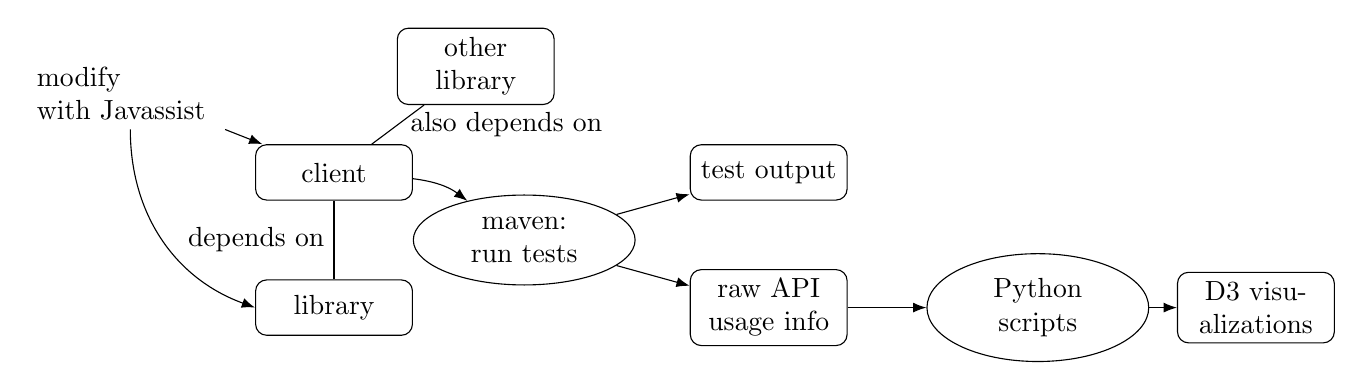
\begin{tikzpicture}
    \node[block] (client) {client};
    \node[block,below=1cm of client] (library) {library};

    \draw (library) -- node[left] (depends) {depends on} (client);

    \node[above left=.75em of client] (ja) {\begin{minipage}{7em} modify \\with Javassist \end{minipage}};
    \draw[-Latex] (ja) -> (client);
    \draw[-Latex] (ja) to [->,bend right=35] (library.west);

    \node[block, above right=2em of client,xshift=-2em] (olib) {other library};
    \draw (client) -- node[right,xshift=.1em] (also) {also depends on} (olib);

    \node[oval,right=of depends] (test) {maven: run tests};

    \draw[-Latex] (client) to [->,bend left=15] (test);

    \node[block, right=10em of client] (output) {test output};
    \node[block, right=10em of library] (raw) {raw API usage info};

    \draw[-Latex] (test) to (output);
    \draw[-Latex] (test) to (raw);

    \node[oval, right=of raw] (Py) {Python scripts};
    \draw[-Latex] (raw) to (Py);

    \node[block, right=1em of Py] (viz) {D3 visualizations};
    \draw[-Latex] (Py) to (viz);
  \end{tikzpicture}
}
  \caption{Our instrumentation workflow. Using Javassist, we analyze and instrument clients and run their test suites. (We process the generated data with Python scripts to create D3 visualizations for VizAPI.)}
  \label{fig:workflow}
 \end{center}
\end{figure*}

Figure~\ref{fig:workflow} summarizes our instrumentation and
data capture workflow. We next describe our instrumentation implementation in detail.

We identify interactions across the client/library boundaries by inspecting JAR files of
each software component to obtain a list of classes for every component. We associate classes 
and their members to components based on these lists. Since the JAR files contain source code,
we ensure that none of the library uses meant solely for unit testing are captured.

\paragraph{Vanilla invocations}
The standard case is simple. At every invoke instruction in every
loaded method which transfers control between the client and the
library, we add code to record that invoke by incrementing a counter.
We handle both static and virtual (including special, virtual,
interface, and dynamic) calls. Crossing the client/library boundary
includes conventional calls from the client to the library as well as callbacks from the library to the client.  

\paragraph{Field accesses}
We capture direct (field sets and gets) and reflective (via invocations of
\texttt{java.lang.reflect.Field.get()} and \texttt{.set()}) field
accesses.

\paragraph{Dynamic proxies and reflective calls}
We specially handle invocations of the distinguished method 
\texttt{java.lang.reflect.Method.invoke()} method used to invoke dynamic proxies and reflective calls, recording
details of the calls that we intercept. 
We identify dynamic proxies by checking whether the invocation 
of \texttt{Method.invoke()} originates from a class that implements 
\texttt{java.lang.reflect.InvocationHandler}. If so,
we inspect the call stack to find the caller and callee of 
\texttt{Method.invoke()} and record the call if it crosses the client/library boundary. 
All other calls to \texttt{Method.invoke()} are standard reflective calls, 
and we record the respective callers and callees.
(We also specifically ignore calls to \texttt{Method.invoke()} made by the Maven surefire plugin
as it runs tests.)
% \todo[inline]{When running tests, the Maven surefire plugin uses the invoke method too,
% which is ignored. Should we talk about that?}

Instrumenting methods also allows us to capture several other library uses,
as we describe below.

\paragraph{Class usages}
We capture reflective uses of the \texttt{Class} object by intercepting calls to
\texttt{java.lang.Class.forName()} and \texttt{java.lang.ClassLoader.loadClass()}.

\paragraph{Service Loaders} We are particularly interested in bypasses of 
services that use the \texttt{ServiceLoader} API. Before the instrumentation, we record a list 
of services and their implementations by inspecting files in \texttt{src/main/resources/META-INF/services}.
With this information, we look for service bypasses which are direct uses of service implementation 
classes in clients, either through instantiations, casts or reflection. We also intercept calls 
to method \texttt{load()} in classes with name \texttt{Service*Loader} and record any calls to methods beyond 
the published interface.

\paragraph{setAccessible()} 
Java provides the \texttt{setAccessible()} method to allow reflective access to class members despite
access modifiers. After a call to this method, the program may then (subject to security manager restrictions)
reflectively access the class member.
We thus record calls to \texttt{setAccessible()} along with the previous visibility of the class member.

\paragraph{Annotations} 
We have a quasi-static approach for finding class, field and method
annotations: we observe all annotations for a class or class member
when it is loaded, and record cases where a class or member declares an
annotation from the library of interest. We also record an association
between the class and its memers' annotations.

\paragraph{Inheritance and interface implementation} At load time,
we also record information about all superclasses and implemented interfaces
that cross the library/client barrier.

\paragraph{Instantiations and casts} We also instrument the
\texttt{NewExpr} and \texttt{Cast} bytecodes to record library/client 
instantiations and casts.

\section{Design Decisions}
\label{sec:design-decisions}

Having described VizAPI's implementation, we now broaden our attention
and discuss possible design alternatives, particularly in terms of toolkits
that we could have used.

As mentioned in Section~\ref{sec:implementation}, VizAPI presents both
static and dynamic information. Static analysis will typically present
over-approximations (e.g. both branches of a conditional might be
taken), except for under-approximations in special cases like
reflection and ``eval''. VizAPI makes almost maximally coarse
over-approximations, for instance by using Class Hierarchy Analysis to
approximate method calls. The soundiness
manifesto~\cite{livshits15:_in_defen_sound} discusses the
underapproximations used by typical static analysis in more detail.

On the other hand, dynamic analysis under-approximates possible
program behaviours: it reports only the behaviour that is induced by
a particular program input. It completely reports that behaviour, though,
and sees through constructs that are difficult for static analyses to
handle soundly. TamiFlex~\cite{bodden11:_tamin_reflec} dynamically captures
information about, for instance, which classes are loaded at runtime,
and feeds that back to the static analysis.

VizAPI integrates static and dynamic information. The approach is
still not sound with respect to all potential executions, and it does
not integrate dynamic class loading information into the static
results, but it does make both types of information (as directly
captured by the tool) visible to the user.

\subsection{Static analysis and program transformation}
We next describe potential static analysis and transformation
approaches, from low-level bytecode manipulation through to
declaratively declaring desired analysis facts. VizAPI extracts static
facts from the programs under analysis. VizAPI also carries out some
program transformation so that it can collect dynamic facts.

Java bytecode is commonly used by program analysis tools as an input
format, since it is widely available and yet preserves the semantics
of the original source code. Unless obfuscated, it contains some
source-level entities such as classes and methods, with their original
names.

Although some source-level information information is present, it is
not complete. Original code structure (e.g. structured Abstract Syntax
Tree-level source-level loops rather than control-flow graphs) and
local variable names may not be present. Hoever, the code structure
can be recovered, and local variable names can be inferred using Big
Code techniques similar to those used for JavaScript by Raychev et
al~\cite{raychev2016learning}.

Bytecode tools provide varying levels of abstraction. We discuss three
bytecode-level tools here, first from the perspective of fact extraction
and then from that of code manipulation and creation.

\paragraph{Low-level analyses}
The Apache Commons Byte Code Engineering Library\footnote{\url{https://commons.apache.org/proper/commons-bcel/}} (BCEL) is a low-level library that
provides a very thin abstraction layer to its user. In particular,
it requires users to manually manage constant pool entries and provides
verbatim access to stack-based bytecode instructions. In that sense,
users need to re-invent the wheel to use it.

The ASM library\footnote{\url{https://asm.ow2.io/}} provides many of
the same capabilities as BCEL, but also a more robust
abstraction layer. For example, ASM manages the constant pool
itself. In addition to an object-oriented (``tree-based'') API like
that of BCEL, it also provides an event-based API which trades increased
performance for decreased flexibility for the user (they must write
the analysis code in a certain way).

We chose to use
Javassist\footnote{\url{https://www.javassist.org/}}~\cite{chiba00:_load_struc_reflec_java}
for VizAPI. It provides more of an abstraction layer than BCEL (no
constant pool) but fewer abstractions than ASM (only one API, not
two). For our purposes, any of the libraries would have
worked, though BCEL would have required more effort to use. \todo{are we sure?}

At a higher (non-bytecode) level, the Soot
framework~\cite{lam11:_soot_java} provides more support for
sophisticated intraprocedural analyses: instead of having to work with
stack-based bytecode, it transforms the input bytecode into a typed
three-address code, with explicit arguments for instructions. Soot
also provides a framework for writing intraprocedural dataflow
analyses.  At the intraprocedural level, because of the three-address
code and the dataflow analysis framework, writing a sophisticated
analysis is far easier in Soot than in bytecode-level libraries. On
the other hand, transforming the code to three-address code involves
more computational overhead.

To provide a concrete example, it is relatively easy to detect method
invocations in all of these frameworks. It is more difficult to, for
instance, detect method invocations with constant parameters, because
the analysis has to reason about the stack contents at the invocation
site. Soot's three-address code hides the stack from the user. In VizAPI's
case, we only need to detect the method invocation, which is easy
with any framework.

\paragraph{Low-level transformation}
While VizAPI's use case includes separate transformation and execution
phases, some tools transform code on-the-fly. All of BCEL, ASM,
and Javassist allow their users to transform code just before executing it,
in the same Virtual Machine. Soot was not designed to support on-the-fly
transformations.

In terms of generating code, the frameworks vary in their API support.
ASM and BCEL provide APIs that require the user to specify the exact
bytecode instructions to be used. Soot allows the user to provide
three-address code instructions by (somewhat awkwardly) constructing
them through its API. Javassist provides a ``simple Java compiler''
which can compile some code fragments into bytecode; the compiler does
not support all Java constructs.  The ByteBuddy
toolkit\footnote{\url{https://bytebuddy.net/}} builds on ASM but
supports a more declarative way of specifying code, e.g. ``create a
method that returns X''.

\paragraph{Interprocedural considerations}
More sophisticated static analysis can benefit from interprocedural
information. For instance, it is useful to know about possible
definition points for a local variable, even when that variable
was assigned from a method parameter.

Unfortunately, in Java, precise interprocedural analysis requires a
call graph and pointer analysis information, and, as pointed out by
Lhot\'ak, call graphs and pointer analysis information must be
computed in tandem. Getting more precise results than Class Hierarchy
Analysis or, perhaps, Rapid Type
Analysis~\cite{bacon96:_fast_static_analy_c_virtual_funct_calls},
requires significant computation, and most analysis users would
benefit from using an off-the-shelf implementation. Soot's SPARK
toolkit is still used today, and
Doop~\cite{bravenboer09:_stric_declar_specif_sophis_point_analy}
provides more sophisticated options, which we discuss shortly.

Assuming that we have a call graph available, the next challenge in
designing a tool is to correctly propagate data interprocedurally.
Even with Soot's call graph information, it is still not that easy to
do whole-program analyses: it is up to the user to manually propagate
information at method invocation sites.

Heros~\cite{bodden12:_inter_proced_data_flow_analy} implements the
IFDS/IDE framework for interprocedural analysis of Java code. Being
interprocedural, it is more complicated to use than the dataflow analysis
framework built into Soot.

To our knowledge, all call graph implementations for Java require
minutes of startup time, even if the call graph computation itself
could be relatively fast. Such analyses would not be appropriate for
use at runtime. (But, any runtime analysis could use dynamic
information and could roll back unsound assumptions that it might have
made).

Also, note that these interprocedural analyses need to know about
program entry points.  For an application with a \texttt{main()}
function, this is straightforward.  For Web middleware or for a
library, this is more complicated, and the user will need to specify
entry points. VizAPI's test-based dynamic approach essentially uses
all test cases as potential entry points, and it is relatively
straightforward to generate a driver that invokes all test cases.

\paragraph{Declarative approaches}
So far, we have discussed analysis and transformation approaches that have
been primarily imperative, with ByteBuddy a minor exception. By contrast,
declarative approaches like Doop are surprisingly powerful and concise.
In Doop's declarative approach, it suffices to declare the rules that
define the analysis. For instance, this utility rule relates methods
that are the same except that they have different declaring types:

\begin{lstlisting}
.decl SameMethodExceptDeclaringType(m:Method, m0:Method)
SameMethodExceptDeclaringType(m, m0) :-
  Method_SimpleName(m, n),
  Method_SimpleName(m0, n),
  Method_Descriptor(m, d),
  Method_Descriptor(m0, d).
\end{lstlisting}

One challenge of using Doop is that it is not obvious to find
the relations that Doop provides to users; the documentation is
somewhat sparse.

In any case, Doop reads the input program and the analysis definition,
computes necessary pointer and callgraph information, and feeds the
facts to the Soufflé Datalog solver. It is fairly simple to read out the
Doop results. Doop does not support program transformation and it would
be challenging to apply Doop results to drive transformations. Doop also
has substantial runtime overhead.

\subsection{Dynamic analysis}

java agent versus JVMTI

Code rewriting


\section{Dataset}
Benchmarks (section 2.3.2 in thesis)

%\section{Results}
\label{sec:results}

We look for our usage patterns in our benchmark collection of 11 libraries (Table~\ref{tab:libs}).

\subsection{API bypasses}
We first investigate the use of API bypasses in our clients. This is useful to library developers if they want to identify which parts of their libraries that are supposed to be internal are actually used by clients. This can help them with API design in future versions. 

In Section~\ref{sec:classification}, we enumerate three broad categories
of bypasses: access modifiers, modularity conventions, and service loaders. We discuss each of them in turn.

%\input{tables/results/set-accessible-client-to-lib}
%\input{tables/results/set-accessible-lib-to-client}

\paragraph{Access modifiers and reflection}
Table~\ref{tab:set-accessible-client-to-lib}
shows selected uses of the reflection API \texttt{setAccessible()} to enable reflective access from clients to libraries,
and Table~\ref{tab:set-accessible-lib-to-client} shows selected uses of \texttt{setAccessible()} to enable reflective callbacks from libraries back to clients.
We can see that accesses to fields, constructors, and methods are all reasonably common, though some codebases only reflectively 
access fields, while others only access methods.

In our data, 1.9\% of the \texttt{setAccessible()} calls are 
used to ensure accessibility of a class member
in the same \texttt{rocketmq} project version 4.9.1 but in a different module (Maven module). 
For instance, \texttt{rocketmq-acl} makes private field \texttt{SendMessageRequestHeaderV2::a} from 
\texttt{rocketmq-common} accessible before accessing it. Such inter-module accesses are more controlled than client/library accesses since they are within the same project,
but are still a form of technical debt.

We investigated all \texttt{setAccessible()} calls on fields that belong to in \emph{rocketmq}. (\emph{rocketmq} is a client that calls \emph{fastjson}). These calls are made from the library to the client, i.e., accesses are from library \emph{fastjson} to client \emph{rocketmq} using callbacks. We see hundreds of \texttt{setAccessible()} calls being executed when the client tests are run. The \emph{rocketmq} source code shows 6 classes with calls to \texttt{setAccessible()}: a serialization/deserialization pair for the \texttt{CommandCustomHeader} class, 2 methods which appear to print out the state of an object for debugging or logging purposes, and 2 methods which store a reference to a specified field or which call a specified method, provided in those methods' parameters. We would not characterize the first 4 API bypasses as misuses, and it is not obvious that the last 2 are misuses either. Another interesting use of \texttt{setAccessible()} on a field is by \emph{benchmark-thrift} to access the field \texttt{maxLength\_}  which is a class member of the class \texttt{TFramedTransport} belonging to Apache \emph{thrift}. This is a private field and the default maximum length is overridden by the client.

We found that 23\% of the calls to \texttt{setAccessible()} were on methods. Of those, only 2 distinct methods that were reflectively invoked were previously not accessible. We manually inspected all of the reflective callers of these 2 methods. Protected method \texttt{Node.setParentNode()} in \emph{jsoup} is called from code in \texttt{org.seimicrawler.xpath} in \emph{JsoupXpath}. This appears to be test code committed to the main repository. The next method is the default-visibility method \texttt{getInstance()}. This method is used to obtain a singleton instance of {\tt ReflectionNavigator} from within the same project. The motivation for developers calling \texttt{setAccessible} within the same project is unclear to us, rather than modifying the code themselves. This work can help developers identify such instances and possibly refactor their code.

We do find that some methods are already accessible before being invoked, and some methods are made accessible but never actually invoked.

An API bypass requires a \texttt{setAccessible()} call followed by an
actual reflective access.  As expected, we see a good overlap between the
\texttt{setAccessible()} calls to methods and reflective invocations.
We find that our benchmarks contain reflective invocations of 20 constructors following a call to \texttt{setAccessible}, which were not already public. Of the 20 callsites, some are generated by the
groovy dynamic language; some are for serialization and some instantiate objects where the constructor had default visibility. All of these reflective constructor invocations are callbacks from the library to the client: the library is providing a factory method to create instances of a client type that it has been supplied with. This appears to be an acceptable API use.
Tables~\ref{tab:refl-fields} and \ref{tab:refl-callbacks} show how many reflective usages are actually made.

Table~\ref{tab:refl-fields} shows some of our data on reflective field accesses. We observe that many of these reflective field accesses are for serialization. We also observe that in the case of fields, there are only a few calls that access fields that were previously not accessible.
%\input{tables/results/reflective-fields}

Table~\ref{tab:refl-callbacks} shows the reflective callback API usage pattern. We see that most accesses in this pattern are made on public methods. We examined the list of methods that are accessed using this usage pattern and this pattern is popular for logging, serialization and deserialization. We also observe a lot of getters and setters accessed this way.



%\input{tables/results/reflective-invocations-client-to-lib}


%% facts about methods:
%% # 827
%% protected 1 org.seimicrawler.xpath.core.node.Text$1::head(Lorg/jsoup/nodes/Node;I)V to org.jsoup.nodes.Node::setParentNode(Lorg/jsoup/nodes/Node;)V, looks like test code
%% default 3 com.sun.xml.bind:jaxb-core:2.2.11 to com.sun.xml.bind.v2.model.nav.ReflectionNavigator::getInstance()Lcom/sun/xml/bind/v2/model/nav/ReflectionNavigator;

%% many of the other calls are during serialization


%% Similarly, \texttt{setAccessible()} on methods in \emph{fastjson} at the behest of \emph{rocketmq} is on constructors, factory methods, and build methods, in the context of Java Beans. As with the fields, these calls essentially enable serialization and deserialization, and are made from class JavaBeanDeserializer.

%% \todo[inline]{Our hypothesis: setAccessible() on methods is used almost exclusively in tests and in serialization. We can verify this by filtering the setAccessible() method calls and excluding everything with ``Test'' and ``Bean'' in it.}
%\input{tables/results/reflective-callbacks}

\paragraph{Containers, modules, and modularity conventions}
For OSGi, none of our libraries are used by our clients in the context of OSGi containers, so the clients are free to violate OSGi access control. Our results show that, even though they can, they almost universally do not. The sole exception is a pair of calls from client \texttt{xsoup} to internal class \texttt{StringUtil} of library \texttt{jsoup}; the calling class in \texttt{xsoup} was copied from \texttt{jsoup} and still uses its internal helper functions. These calls violate both modularity conventions and OSGi export declarations. When we found these calls, we submitted a pull request\footnote{https://github.com/code4craft/xsoup/pull/53} duplicating the \texttt{jsoup} methods into \texttt{xsoup}, and it was quickly merged, showing that the \texttt{xsoup} developer was not in favour of violating modularity conventions.
% https://github.com/code4craft/xsoup/pull/53

Similarly, although we have Java 8 clients which can violate the unenforced module export rules of Java 9 libraries (they run in environments that don't enforce the rules), none of the clients do so. We believe that the most likely explanation is that such modularity violations are uncommon; however, it is also possible that Java 9 module definitions are too permissive and do not prevent calls that should be prevented.

Table~\ref{tab:internal} shows uses of packages labelled ``internal'' from outside
a given module. In some cases (for example, netty-buffer and netty-common),
the uses are across different modules in the same project. We looked
at one case, \emph{rocketmq-remoting} and \emph{netty}. In this case,
\emph{rocketmq-remoting} uses internal logging infrastructure from
\emph{netty} in its NettyLogger module; such a module might be
expected to be more closely coupled to its callee than other parts of
the code. On the other hand, the usage of \emph{groovy} internals in
\emph{rest-assured} would appear to be due to the choice of Groovy as
an implementation language, and thus compiler-generated references to
internals in the \emph{rest-assured} code.

%\input{tables/results/internal}


\paragraph{Service bypasses}
We find that all clients of libraries that use service loaders bypass the defined services. This is done most commonly through instantiation, but also through casts, subtyping and reflection.

For instance, component \emph{com.h2database:h2} advertises a service (\texttt{org.h2.Driver} implementing \texttt{java.sql.Driver}), making it a JDBC4-compliant driver. Its clients can obtain connections through the JDBC driver manager, which selects and instantiates instances based on driver URLs. However, client \texttt{glowroot.agent} (specifically class \texttt{org.glowroot.\-agent.embedded.util.DataSource}) directly instantiates \texttt{org.h2.jdbc.JdbcConnection} and therefore becomes dependent on using the particular database \emph{h2}. This leads to further direct calls to \texttt{org.h2.jdbc} APIs being observed. This is a clear bypass of a defined API. 

Now consider \emph{fastjson}. This component declares that it provides several services, including three services defined by interfaces in the \texttt{javax.ws.rs.ext} package, part of the JEE support for RESTful services. 
The respective services are implemented in classes in the package \texttt{com.alibaba.fastjson.support.jaxrs}.   
However, looking at clients, we also see calls to APIs provided in \emph{fastjson} APIs outside packages implementing the interfaces declared as services. For instance, \texttt{com.alibaba.fastjson.JSON::toJSONString} is called from \texttt{org.springframework:spring-web}.
%:4.3.7.RELEASE.    
This is a legitimate use of a JSON parser via a non-standard API, and in this sense, it is a false positive as we detect it as a API misuse. So \emph{fastjson} could be easily split into two components, one providing an ``open API'' for the JSON parser functionality, and one implementing and providing the RESTful services. The services would then depend on the open API. This would significantly reduce the overall API surface of fastjson, splitting it into two components, each with well defined functionalities and internal coherence.

We have mainly focussed on ``why not'', i.e. what mechanisms clients use to bypass API restrictions: reflection, violating conventions, and service loader bypasses, and reported results with respect to ``what thing''. When relevant, we discussed ``how'' the bypass occurred, especially for reflection, and we reported the directionality of the bypasses.

\begin{mdframed}[
  leftmargin=\parindent,
  rightmargin=\parindent,
  skipabove=\topsep,
  skipbelow=\topsep
  ]
{\bf Finding 1:} Programs are generally well-behaved: reflection is mostly used for serialization not API bypasses; OSGi and Java 9 module definitions are always respected; internal packages are only called sparingly; but service loaders are almost always bypassed.
\end{mdframed}

\subsection{Extent of API usage}
Continuing with our investigation of API surfaces, but moving from
misuses to uses, we present results on API use.
%, again using results obtained from our instrumentation.

Table~\ref{tab:usage-distribution} presents the usage distribution of
libraries' API elements (methods, fields, and classes subtyped) as
covered by client tests. The ``total in lib'' refers to the number of
public and protected members, including static ones. To calculate these totals,
we use the latest stable version of each library and consider it to be representative of 
the versions used by clients.  The ``distinct used'' column counts an
element once regardless of how many clients use that element, while
``total used'' counts an element once per client using it. We identify method calls by the
declared type of the receiver object, for example, calls to {\tt o1.f()} and {\tt o2.f()} are the same
if {\tt o1} and {\tt o2} have the same declared type.
Our uses 
include both vanilla and reflective uses of API elements.

%\input{tables/results/standard-api-usage}

We can observe that at most 22\% (and on average 9\%) of the methods in the API surface
are used by clients, with \emph{slf4j-api} having the highest use proportion.
% , and sometimes less than 1\%  of methods. 
Table~\ref{tab:usage-distribution} suggests that there is a small overlap between methods
used by clients.

We also looked at the \emph{json} library and found that its own tests reach 151
of the 258 API methods, compared to the 25 methods used by our selected
clients. One possible reason for the sparsity of API use is that, at least in \emph{json}, over half of the API methods are overloaded, i.e. share a name with
some other API method.

% reads or writes would be nice to know, but we can't get it in time.
Despite standard OO practices calling for fields to be encapsulated, more than half of the libraries have their fields accessed by clients. Only 1 of the \emph{joda-time} and 25 of the \emph{jackson-core} fields are static (so it's not just constants); the rest of the accesses are to instance fields.
However, the number of fields used is often in the single digits,
the \emph{jackson} libraries being an exception with about 11\% of declared fields used.
We inspected the use of \emph{jackson} fields and found that these usages mostly exist within the \emph{jackson} libraries themselves.
We count calls that happen across the \emph{jackson} libraries as crossing library/client boundaries.
An example of these usages is the {\tt WritableTypeId} class belonging to \emph{jackson-core}, which is used often, and usually by \emph{jackson-databind}.
{\tt WritableTypeId} is a Java class that acts like a C-style struct; it exposes fields and not methods. It is intended to be used for passing information, and the use of its fields is expected.

About half of the libraries have clients subclassing a
single-digit number of library types, again with the exception of
\emph{jackson} with dozens of subtypes in clients, which are also often other \emph{jackson} libraries.

We observe only one use of library annotations across all our benchmarks. \emph{crushpaper} uses \texttt{com.fasterxml.jackson.databind.annotation.JacksonStdImpl}, which is used for indicating implementation classes and is typically used by serializers and deserializers in \emph{jackson}.

Figure~\ref{fig:jaccard} presents a boxplot of
pairwise Jaccard similarities between the portion of
the APIs used by different clients for each library. Two clients $u_1$ and $u_2$ 
of library $L$ which use exactly the same parts of $L$'s API would result in a similarity of 1;
more generally, it is
\[ \frac{|\mbox{used.API}_L(u_1) \cap \mbox{used.API}_L(u_2)|}{|\mbox{used.API}_L(u_1) \cup \mbox{used.API}_L(u_2)|}. \]

Although Table~\ref{tab:usage-distribution} showed that some of the members overlap, we can
see from this Figure that the overall level of overlap is generally less than 10\%. We observe
a half-dozen client pairs (data points) where there is about 50\% overlap between client API uses, including for \emph{fastjson},
\emph{commons-io}, and \emph{json}. Although the mean overlap for \emph{slf4j-api} is near 0, there are also 4 pairs of clients which have more than 50\% overlap.

\begin{center}
\begin{figure}
\centering
%\includegraphics[width=8cm, height=7cm]{./images/jac-sim-box-plot-declared}
\caption{\label{fig:jaccard}Jaccard similarities between clients' API usages}
\end{figure}
\end{center}
%% Digging into \emph{fastjson}, we found that it is a ``mixed type'' library: some clients use APIs related
%% to \texttt{javax.ws.rs}, the JEE standard for restful services, while others use just a standalone parser API that does not implement an external specification. 

We were not surprised by the generally small amounts of overlap, because the libraries' exposed API surfaces tended
to have thousands of exposed elements and hundreds of used elements. This result makes a convincing argument for libraries being fissioned into modules, which we discuss further in Section~\ref{sec:fission}. 

Table~\ref{tab:same-method} presents another view of API overlap between clients. We constructed the largest set
of methods shared by more than 1 client of a library (``max-set'') and report the size of that set as well as the percentage
of clients which use all of that set of methods. So, for \emph{json}, we can see that there is one method called
by 3 out of 4 clients, and for \emph{jsoup}, ten methods are all called
by 3 out of 4 clients. We characterize the amount of overlap as generally low but not
nonexistent: a few methods are repeatedly used.

%\input{tables/results/perc-clients-same-methods}

%{\bf Research Question 2.} (a) Do clients often use only a subset of the published API? How big is this subset? (b) For each library, is that subset consistent across clients? (c) Do different libraries show different usage patterns by clients?

\begin{mdframed}[
  leftmargin=\parindent,
  rightmargin=\parindent,
  skipabove=\topsep,
  skipbelow=\topsep
  ]
{\bf Finding 2:} APIs are sparsely used by clients---mostly methods (9\% utilization), but a few fields (4\%) and supertypes (6\%). There is limited but nonzero overlap between the methods used by different clients.
\end{mdframed}

\section{Potential Applications}
Potential Applications:
Security: 
Identify illegal accesses and abnormal usage
Identify propagated vulnerabilities from dependencies
Developer experience: analyze dataset for improving experience of library users
Help library developers identify which features to focus efforts on
Predict good choices of libraries based on client use case
Analyze library version usage
How does static and dynamic usage differ?
(other ML applications of the data??)

\section{Conclusion}



WASM, the Java Bytecode of the 2020s.



%% The Appendices part is started with the command \appendix;
%% appendix sections are then done as normal sections
%% \appendix

%% \section{}
%% \label{}

%% References
%%
%% Following citation commands can be used in the body text:
%% Usage of \cite is as follows:
%%   \cite{key}         ==>>  [#]
%%   \cite[chap. 2]{key} ==>> [#, chap. 2]
%%

%% References with BibTeX database:

\bibliographystyle{elsarticle-num}
\bibliography{main}


\end{document}

%%
%% End of file `ecrc-template.tex'. 
